%-*-coding: utf-8-*-

\graphicspath{ {images/} }

\startrelatedwork

\chapter{Обзор предметной области}
В данной главе проводится обзор предметной области.
Дается объяснение технологии "блокчейн", а также данных, которые хранятся в нем.
Далее приводится объяснение консенсус алгоритма, рассмотрение основных их типов и их недостатков, далее идут технические детали о транзакциях, хранилище и используемых криптографических алгоритмов.

TODO лел

\section{Технология блокчейн}

Технология блокчейн, от английского blockchain, дословно переводится  как "цепочка блоков".

Блок хранит в себе данные, а также ссылку на предыдущий блок. 
Блоки образуют бесконечную последовательность, которая имеет начало, но не имеет конца.
Первый блок в блокчейне называется \textit{генезис} блоком (от английского genesis - зарождение).

По сути блокченй представляет односвязный список, где каждый элемент знает ссылку на предыдущий. 
Однако, особенностью данного списка является то,  что в качестве ссылки на предыдущий блок 
используется хэш криптографически стойкой хэш-функции содержимого предыдущего блока, 
которое включает как его данные, так и ссылку на предыдущий блок. 
Поэтому при даже малейшей попытке заменить содержимое блока, 
поменяется значение хэш-функции его данных и ссылка на него от последующего блока будет недействительна.
Нахождение двух блоков с разным содержанием и одинаковым значением хэш-функции является NP-полной задачей.
Данная особенность ключевая, и  является основной для обеспечения безопасности в криптовалютах использующих технологию блокчейн.

\begin{figure}[h]
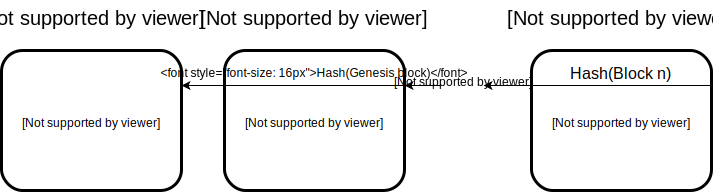
\includegraphics[scale=0.6]{Blockchain_Scheme}
\caption{\textbf{Схема блокчейна}}
\label{fig:blockchain}
\end{figure}

TODO схематичное представление блокчейна

Формально блокчейн можно описать следующей системой формул.

TODO формулы

Будем называть описанную структуру - блокчейн.

\section{Алгоритм консенсуса}

\section{Транзакции и хранилище}
В данном разделе будут введены понятия транзакции и хранилища. 

Основной функционал в криптовалюте - это возможность переводить другим участникам системы средства, а также получать средства на свой счет.
Чтобы понять, как это реализовано, разобремся как хранится информация о счетах и как производится перевод средств между ними.

У каждого участника системы имеется \textit{адрес} TODO, на котором хранятся его \textit{токены}, токены
являются аналогом фиатной валюты, например рубля или доллара . Количество токенов участника на его адресе будем называть \textit{балансом}. Токены между адресами пересылаются с помощью \textit{транзакции}. Транзакция - это подтвержденное криптографической подписью сообщение, которое указывает с каких и на какие адреса отправлять и получать токены, а также количество токенов. Более точное содержимое транзакции будет описано далее в этом разделе.

Вся информация о балансах хранится в базе данных, которую в рамках данной работы будет называться \textit{хранилищем}.
Данная база данных может быть распределенной, тогда части ее будут храниться на устройствах участников системы. 
Такой подход называется шардирование (от английского sharding). 
Другой, более простой подход, состоит в том, что копия этой базы данных хранится у каждого участника системы.
В данной работе будет использоваться этот более простой подход.

Существует несколько различных способов организации хранилища.
Такое разнообразие обсусловлено стремлением побороться  с проблемой double-spending[ссылка].
Мы рассмотрим два самых распространненный способа. 
Однаков, в рамках данной работы не принципиально, какой из способов будет использоваться в реализации.

\subsection{Хранилище на основе списка адресов}
Обозначим через $\boldsymbol{\sigma}$ отображение из адреса в состояние адреса. Тогда для адреса $a$ в $\boldsymbol{\sigma}[a]$ содержится:
\begin{itemize}
\item balance - целая величина, количество токенов принадлежащих адресу $a$
\item nonce  - целая величина, количество транзакций отправленных с этого адреса
\end{itemize}

nonce хранится для того, чтобы предотвратить проблему double-spending. 

\noindent Транзакция содержит следующие данные:
\begin{itemize}
\item $s$ - адрес отправителя
\item $r$ - адрес получателя
\item $n$ - nonce адрес отправителя в момент создания транзакции
\item $amount$ - количество переводимых токенов
\item $pk$ - публичный ключ отправителя (sender)
\item $sig$ - подпись кортежа $(s, r, amount, n)$, сделанная с помощью секретного ключа $s$
\end{itemize}

\noindent Таким образом, каждый участник системы может проверить, что подпись действительно сделана с помощью секретного ключа, соответствующего публичному ключу pk. Попытка подделать кортеж $(s, r, amount, n)$, чтобы подпись осталась такой же, является NP полной задачей.

После того как участник системы получает транзакцию $t$, он проверяет, что выполняются следующие условия:
\begin{itemize}
\item $\boldsymbol{\sigma}[s].balance \ge t.amount$ - отправитель имеет достаточное количество токенов
\item $\boldsymbol{\sigma}[s].nonce = t.n$ - nonce транзакции совпадает с хранимым в хранилище
\item $verifySignature(t.sig, t.pk, (t.s, t.r, t.amount, t.n))$ - подпись в транзакции корректна
\end{itemize}

Если все вышеописанные условия выполняются, то участник обновляет локальную копию хранилища следующим образом:

$\boldsymbol{\sigma}[s].balance = \boldsymbol{\sigma}[s].balance - t.amount$

$\boldsymbol{\sigma}[r].balance = \boldsymbol{\sigma}[r].balance + t.amount$

$\boldsymbol{\sigma}[s].nonce = \boldsymbol{\sigma}[s].nonce + 1$\\
Все данные изменения должны проводиться атомарно, чтобы избежать неконсистентного состояния хранилища.

\subsection{Хранилище на основе списка непотраченых выходов}

\section{Криптография}

\section{Существующие криптовалюты}

\finishrelatedwork